\documentclass[11pt,a4paper]{article}
\usepackage[utf8x]{inputenc}
\usepackage{amsmath}
\usepackage{amsfonts}
\usepackage{graphicx}
\usepackage[table,xcdraw]{xcolor}

\usepackage{caption}
\usepackage{subcaption}

\renewcommand{\familydefault}{\sfdefault} % cambiamos la fuente a una sans

\usepackage{float} % para que floten las imagenes o algo asi...
\usepackage{wallpaper} %paquete para usar una imagen como encabezado!
\usepackage{hyperref} %para usar hypervinculos 
\usepackage[export]{adjustbox} %para usar marcos en imagenes
\usepackage{eurosym} % para el euro
\usepackage{transparent} %para las marcas de agua
\usepackage{eso-pic}  %para las marcas de agua

\definecolor{azul_marcos}{RGB}{0,128,159} %defino el color azul de los marcos
\usepackage{sectsty} %esto es para cambiar el color de las fuentes creo
\renewcommand{\familydefault}{\sfdefault} % cambiamos la fuente a una sans
\sectionfont{\color{azul_marcos}}  % sets colour of sections
\subsectionfont{\color{azul_marcos}}  % sets colour of sections


\usepackage{pdfpages} %para insertar pdfs
\usepackage{amssymb}
\usepackage{pstcol} % para color
\usepackage{pst-node} % para diagramas
\usepackage{pst-plot} % para representacion de dat
\usepackage[portuguese]{babel}
\addto\captionsspanish{\renewcommand\chaptername{Bloque}}
%\usepackage[total={18cm,21cm},top=2cm, left=2cm]{geometry}
\usepackage{anysize}
\pagestyle{plain}
%\markboth{left head}{right head}
%\markright{Guía de impresión ABS Tech}
\marginsize{3cm}{2cm}{2.5cm}{1cm}
\title{Guía do impressão ABS Tech}
\date{}

%configuracion de la marca de agua
\AddToShipoutPicture{
    \put(0,0){
        \parbox[b][\paperheight]{\paperwidth}{%
            \vfill
            \centering
            {\transparent{0.1}
\includegraphics[scale=1.25]{FOTOS/logofff}}%
            \vfill
        }
    }
}

\begin{document}
\ULCornerWallPaper{1}{FOTOS/header}
\LLCornerWallPaper{1}{FOTOS/footer}
%\maketitle
%\tableofcontents

\includepdf{PDF/PORTADA.pdf}
\section{O que é o filamento ABS Tech?}ABS Tech é um filamento para impressão 3D FFF/FDM de acrilonitrilo butadieno estireno (A.B.S.) especialmente tratado com aditivos para reduzir o efeito warping caraterístico deste material e torná-lo mais fácil de usar.
\section{Porquê usar ABS Tech?}
ABS Tech amplía las posibilidades de los filamentos de ABS tradicionales manteniendo a la vez las propiedades químicas y mecánicas de este fantástico termoplástico.
\begin{itemize}
\item O seu tratamento anti-warping permite a impressão de volumes maiores que os habituais e um melhor aproveitamento em impressoras domésticas.
\item Os cheiros produzidos pelo nosso ABS Tech são menos incómodos que os de outros filamentos de ABS.
\item ABS Tech é um material muito tenaz, duro e com boa resistência química à abrasão.
\item É solúvel em acetona. Isto permite unir fortemente peças de ABS usando acetona como aglutinante.
\item Por último as peças impressas em ABS Tech podem processar-se posteriormente com facilidade, já que este material pode ser furado, lixado, pintado, etc...
\end{itemize}
\section{Ficha técnica e parâmetros de impressão}
\begin{table}[H]
\centering
\caption*{Ficha técnica}
\begin{tabular}{|
>{\columncolor[HTML]{FFFFFF}}l |
>{\columncolor[HTML]{FFFFFF}}c |}
\hline
\multicolumn{1}{|c|}{\cellcolor[HTML]{FFFFFF}\textbf{Material}}   & Acrilonitrilo Butadieno Estireno   \\ \hline
\textbf{Cores disponiveis}              & 2                 \\ \hline
\textbf{Formatos disponíveis}             & 1kg, 250gr         \\ \hline
\textbf{Temperatura de deflexão térmica} & 88ºC               \\ \hline
\textbf{Temperatura de fusão}            & 200ºC              \\ \hline
\textbf{Temperatura de decomposição}    & \textgreater 260ºC \\ \hline
\textbf{Densidade}                         & 1.05 gr / cm3      \\ \hline
\textbf{Resistência ao impacto}                         & 17 kg-cm / cm3      \\ \hline
\textbf{Alongamento máximo}              & 25\%              \\ \hline
\end{tabular}
\end{table}
\begin{table}[H]
\centering
\begin{tabular}{|
>{\columncolor[HTML]{FFFFFF}}l |
>{\columncolor[HTML]{FFFFFF}}c |}
\hline
\multicolumn{1}{|c|}{\cellcolor[HTML]{FFFFFF}\textbf{Temperatura de impressão recomendada}} & 240º-245º              \\ \hline
\textbf{Velocidade de impressão recomendada}                         & 50-90mm/s              \\ \hline
\textbf{Temperatura do leito quentes}                                  &  80º - 100º        \\ \hline
\textbf{Camada ventilador}                                      & Off ou baixa velocidade                 \\ \hline
\textbf{Velocidade da primeira camada}                                                 & 20 mm/s                      \\ \hline
\textbf{Altura da primeira camada}                                           & \textgreater 0.2 mm                      \\ \hline
\end{tabular}
\end{table}

Pode descarregar os nossos perfis completos de impressão dos principais programas de laminação (Cura, Slic3r e Simplify3D) no nosso site:
\\\\
\centerline{ {\huge \url{www.fffworld.com/documentation} } }
\\\\
Os parâmetros ótimos dependerão da impressora 3D que você utilize, no entanto, são bons parâmetros para tomar como ponto de partida. Com umas poucas impressões será capaz de encontrar os limites e a configuração perfeita para a sua máquina.
\section{Problemas e soluções}
	\subsection{O warping e o cracking}
		\subsubsection{O que são?}O ABS é um material ideal para imprimir em 3D pela sua disponibilidade e caraterísticas: extrude-se a uma temperatura ligeiramente superior à do PLA, é menos exigente com o tipo de hot-end utilizado, é menos propenso a encravamentos, dado que não se cristaliza ao degradar-se e possui propriedades mecânicas superiores.
\\\\
A sua maior desvantagem é o conhecido efeito warping/craking, no entanto, com os conselhos adequados, estes problemas podem ultrapassar-se.
\\\\
O efeito warping é o nome que recebe no mundo da impressão 3D a problemática causada pela contração do plástico ao arrefecer, o que por vezes provoca que as peças se deformem ou se partam.
\\\\
Distingue-se entre warping e cracking conforme o problema afete a primeira capa ou as capas intermédias da peça.
%EJEMPLO_WARPING
%Leyenda: Ejemplo de problema de warping
%EJEMPLO_CRACKING
%Leyenda: Ejemplo de problema de cracking
\begin{figure}[H]
    \centering
    \begin{subfigure}[b]{0.4\textwidth}
        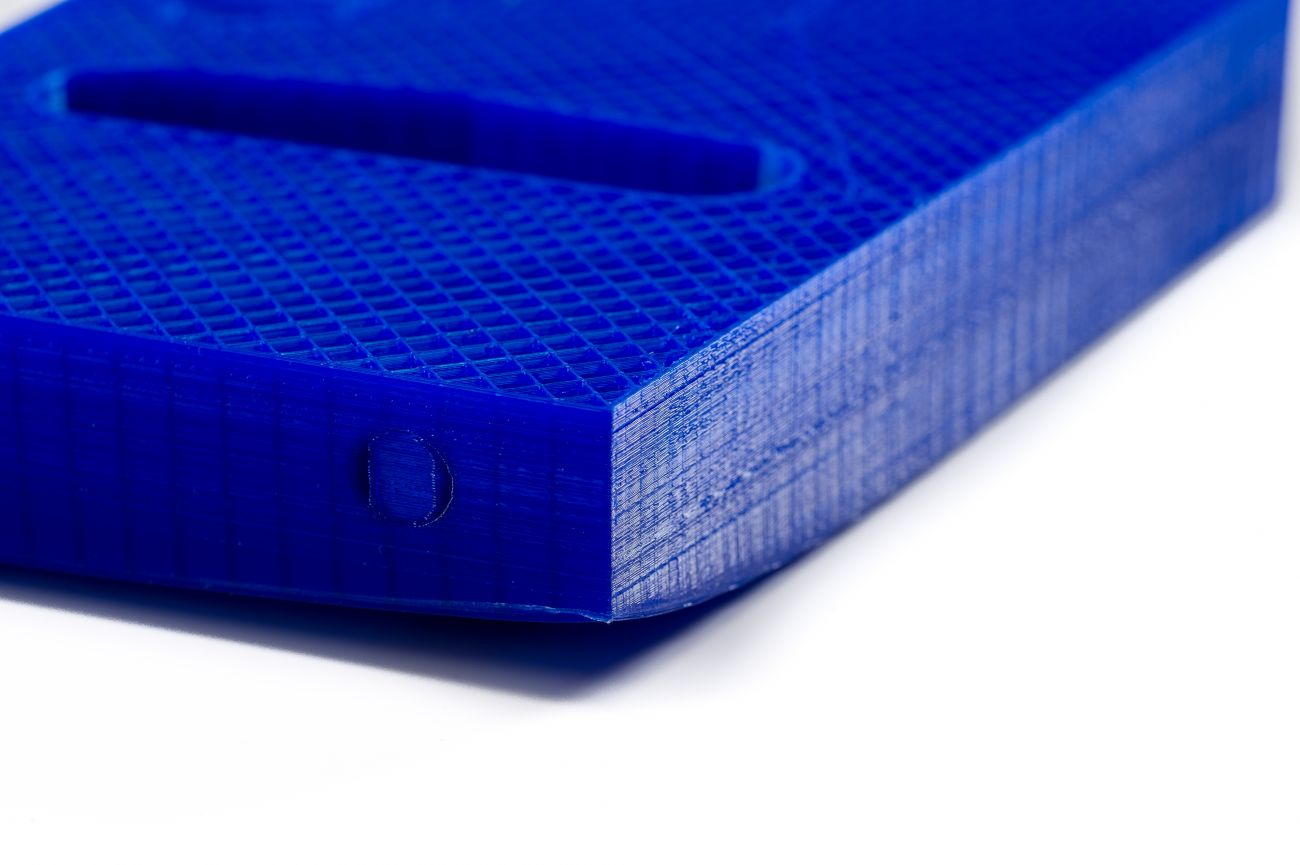
\includegraphics[width=\textwidth,cfbox=azul_marcos 4pt 0pt]{FOTOS/EJEMPLO_WARPING}
	\caption*{Exemplo de problema de warping}
    \end{subfigure}
    \qquad %add desired spacing between images, e. g. ~, \quad, \qquad, \hfill etc. 
      %(or a blank line to force the subfigure onto a new line)
    \begin{subfigure}[b]{0.4\textwidth}
        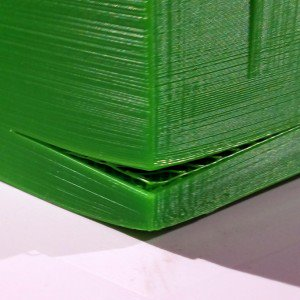
\includegraphics[width=\textwidth,cfbox=azul_marcos 4pt 0pt]{FOTOS/EJEMPLO_CRACKING}
	\caption*{Exemplo de problema de cracking}
    \end{subfigure}   
\end{figure}
		\subsubsection{Quais são as suas causas?}Imprimir em 3D supõe depositar fios de filamento que se pegam entre si e constroem as peças desejadas.
\\\\
Ao arrefecer, estes fios contraem-se, reduzindo o seu comprimento e provocam tensões acumuladas nas peças com efeitos indesejados.
\\\\
As distintas fases do problema podem observar-se na imagem:
%CAUSA WARPING
\begin{figure}[H]
\centering
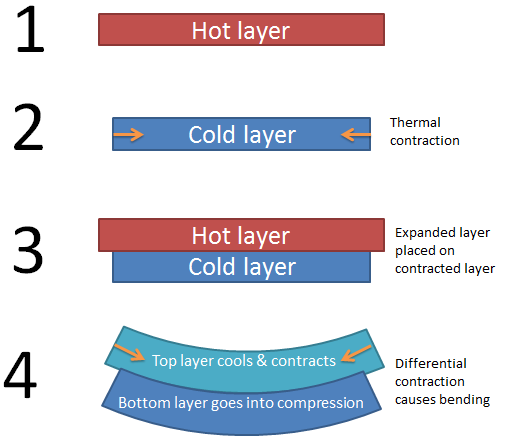
\includegraphics[width=0.6\textwidth,cfbox=azul_marcos 4pt 0pt]{FOTOS/CAUSA_WARPING_1}
\end{figure}

\begin{description}
\item[1] A primeira capa deposita-se quente: Ao estar ainda quente, o seu tamanho é superior ao que terá à temperatura ambiente.
\item[2] A primeira capa arrefece: Ao arrefecer contrai-se, reduzindo-se o seu tamanho, e aparecem as primeiras tensões, que tendem a descolar a peça da superfície de impressão.
\item[3] A segunda capa deposita quente: Ao estar quente, o volume da segunda capa é maior que o da primeira.
\item[4] A segunda capa arrefece: A tensão gerada pela contração da segunda capa acresce à provocada pela primeira capa e a peça descola-se, curvando-se.
\end{description}
			\paragraph{A influência da temperatura no warping}\mbox{}\\\\
A diferença de temperatura é portanto a responsável pelo problema, em concreto a diferença entre a temperatura ambiente e a temperatura de transição vítrea do material.
\\\\
\url{https://en.wikipedia.org/wiki/Glass_transition}
\\\\
A temperatura de transição vítrea do ABS é de cerca de 100º e sendo a temperatura ambiente por volta dos 30º, é esse salto de 70º que provoca o problema.
\\\\
Como curiosidade vale a pena explicar que o PLA se dilata mais que o ABS com a temperatura, no entanto a sua transição vítrea situa-se por volta dos 60º e, como a diferença em relação à temperatura ambiente é muito menor, não se verifica o efeito warping.
\\\\
Portanto, controlando a temperatura ambiente, podemos controlar totalmente o warping, ainda que isto nem sempre seja simples.
		\subsubsection{Soluções físicas}
			\paragraph{Melhorar a aderência da superfície de impressão}\mbox{}\\\\
O efeito warping pode-se atenuar melhorando a aderência da superfície de impressão, contudo, esta não é a melhor solução, dado que não ataca a raiz do problema e não faríamos nada para solucionar o cracking.
\\\\
%CAUSA WARPING 2
\begin{figure}[H]
\centering
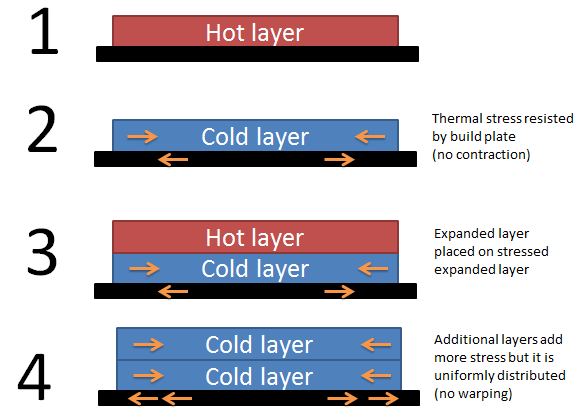
\includegraphics[width=0.6\textwidth,cfbox=azul_marcos 4pt 0pt]{FOTOS/CAUSA_WARPING_2}
\end{figure}

\begin{description}
\item[1] A primeira capa deposita-se quente: Ao estar ainda quente, o seu tamanho é superior ao que terá à temperatura ambiente.
\item[2] A primeira capa arrefece: Ao arrefecer, a primeira capa tende a contrair-se, no entanto a aderência da superfície contraria esta força.
\end{description}
Aplicando um produto adesivo não se eliminarão as tensões produzidas pelo arrefecimento do ABS, mas podem contrariar-se, sendo uma solução eficaz para peças pequenas.
\\\\
É muito importante que a superfície não tenha pó, gordura ou elementos estranhos que afetem negativamente a aderência.
\\\\
Também é necessário que a superfície de impressão esteja perfeitamente nivelada, para que a primeira capa tenha uma altura uniforme.
\\\\
Entre os produtos mais usados e com melhores resultados podemos encontrar:

				\subparagraph{Fita kapton}\mbox{}\\\\
Trata-se de uma fita adesiva de poliamida com adesivo de silicone, preparada para suportar altas temperaturas. O ABS adere bastante bem a este tipo de fita e foi muito utilizada em impressão 3D com este propósito. Para utilizá-la corretamente é necessário colá-la com cuidado à superfície de impressão.
%KAPTON1 KAPTON2
\begin{figure}[H]
    \centering
    \begin{subfigure}[b]{0.4\textwidth}
        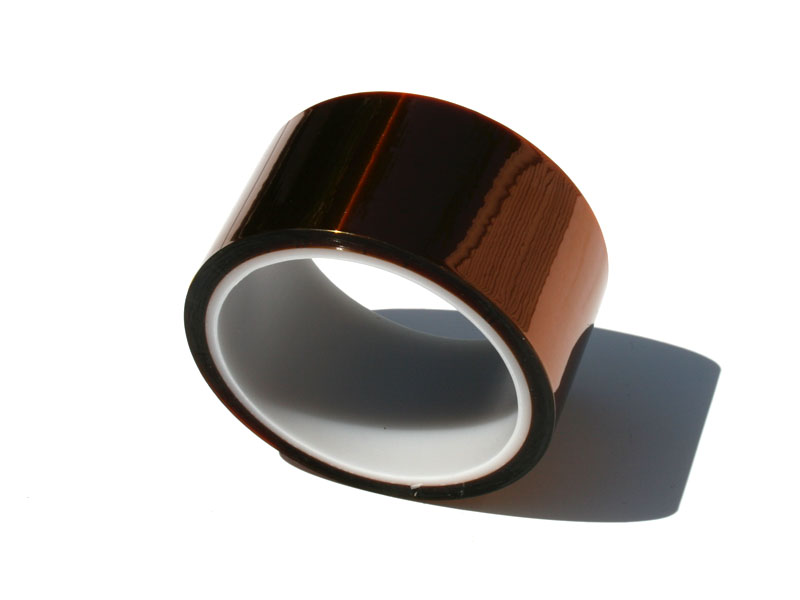
\includegraphics[width=\textwidth,cfbox=azul_marcos 4pt 0pt]{FOTOS/KAPTON1}
	\caption*{Rolo de fita Kapton}
    \end{subfigure}
    \qquad %add desired spacing between images, e. g. ~, \quad, \qquad, \hfill etc. 
      %(or a blank line to force the subfigure onto a new line)
    \begin{subfigure}[b]{0.4\textwidth}
        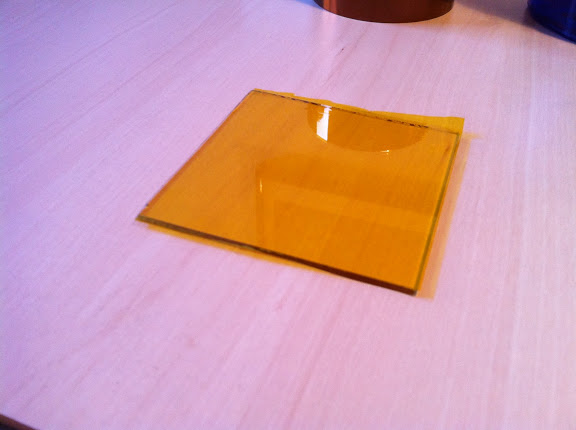
\includegraphics[width=\textwidth,cfbox=azul_marcos 4pt 0pt]{FOTOS/KAPTON2}
	\caption*{Vidro com Kapton}
    \end{subfigure}   
\end{figure}
				\subparagraph{Laca}\mbox{}\\\\
A laca demonstrou ser um recurso eficaz na hora de incrementar a aderência da superfície de impressão. É aconselhável escolher uma laca que contenha o menor número de aditivos possível. A forma de utilizá-la é pulverizar abundantemente a superfície de impressão antes de imprimir.
%LACA
\begin{figure}[H]
\centering
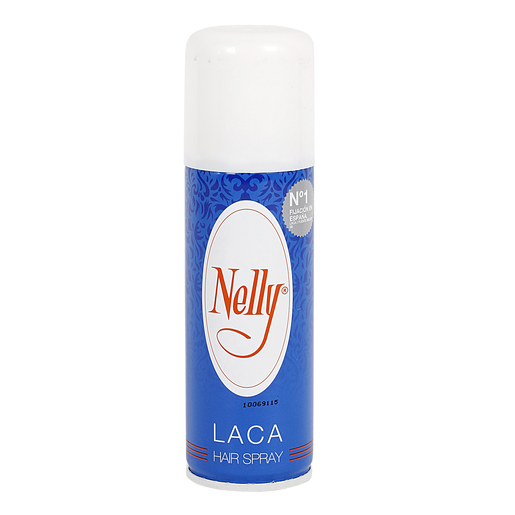
\includegraphics[width=0.3\textwidth,cfbox=azul_marcos 4pt 0pt]{FOTOS/LACA}
\caption*{Laca Nelly}
\end{figure}
				\subparagraph{Dissolução ABS-Acetona}\footnote{ADVERTÊNCIA: Este método pode ser tão eficaz que a peça resultante não possa ser descolada da base sem partir um dos dois} \mbox{}\\\\
Aproveitando a solubilidade do ABS em acetona pode preparar-se uma solução para colar fortemente as peças à superfície de impressão. É necessário mergulhar pedaços de ABS em acetona e deixar que esta dissolva o plástico. Depois de dissolvido, o líquido resultante pode aplicar-se com um pincel sobre a superfície de impressão, para aumentar notavelmente a aderência.
				\subparagraph{Outros produtos}\mbox{}\\\\
Além dos métodos mencionados existem outros para conseguir os mesmos objetivos. Por outro lado, o avanço da impressão 3D propiciou a aparição de produtos específicos para solucionar os problemas de aderência. Consideramos que os métodos anteriormente expostos são os mais acessíveis e eficazes, no entanto queremos mencionar outros que podem ser-lhe úteis:
\begin{description}
\item[Superfícies de impressão] 3M BlueTape, Buildtak
\item[Produtos adesivos] Fixwarp3d, 3DLAC, Dimafix, Colagem com tubo UHU (PVA)
\end{description}
			\paragraph{Utilização de cama quente}\mbox{}\\\\
É necessário utilizar uma superfície de impressão aquecida (cama quente) para imprimir ABS de forma satisfatória e são muitas as impressoras que incorporam una.
\begin{figure}[H]
\centering
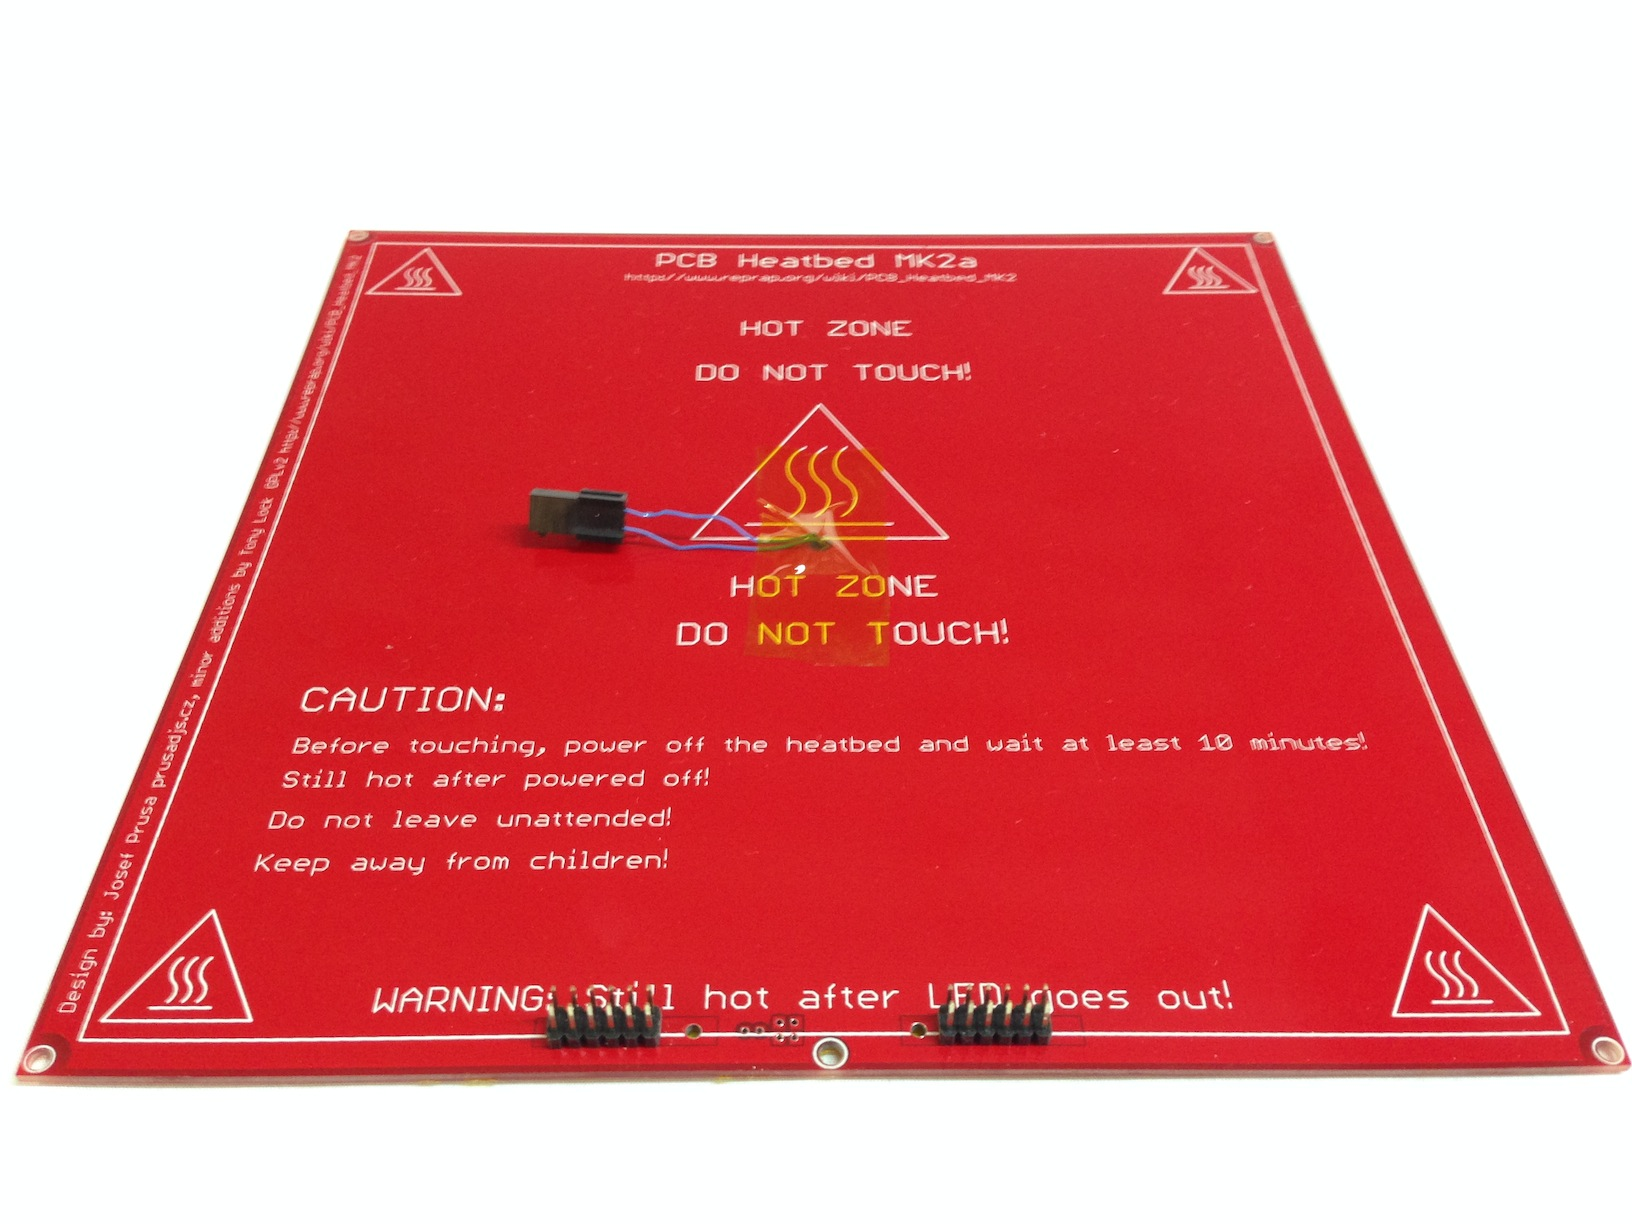
\includegraphics[width=0.6\textwidth,cfbox=azul_marcos 4pt 0pt]{FOTOS/HEATEDBED}
\caption*{Cama quente para impressora RepRap}
\end{figure}
A cama quente vai assegurar que as primeiras capas se mantenham a uma temperatura suficiente para evitar a contração do material e os problemas de warping.
\\\\
A cama quente deve aquecer-se pelo menos a 80º, ainda que seja recomendável que esteja pelo menos a 100º.
\\\\
Deve ter-se em conta que a cama quente não consegue manter a temperatura das capas superiores em peças grandes, portanto pode ainda ocorrer cracking em volumes grandes.
			\paragraph{Evitar correntes de ar}\mbox{}\\\\
Para evitar que a peça possa arrefecer bruscamente é bastante conveniente imprimir em espaços resguardados de correntes de ar. Isto entra em conflito com a recomendação de imprimir em áreas ventiladas para evitar a acumulação de gases nocivos.
\\\\
Portanto, a melhor opção passa por fechar a impressora num recinto que permita manter a temperatura e evitar correntes de ar.
% CERRAMIENTO1  CERRAMIENTO2  CERRAMIENTO3 
\begin{figure}[H]
    \centering
    \begin{subfigure}[b]{0.3\textwidth}
        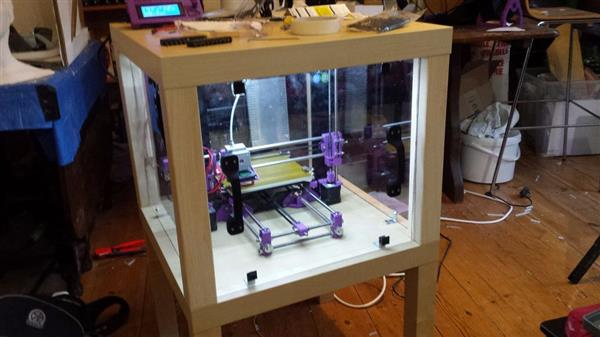
\includegraphics[width=\textwidth,cfbox=azul_marcos 4pt 0pt]{FOTOS/CERRAMIENTO1}
    \end{subfigure}
    \quad %add desired spacing between images, e. g. ~, \quad, \qquad, \hfill etc. 
      %(or a blank line to force the subfigure onto a new line)
    \begin{subfigure}[b]{0.3\textwidth}
        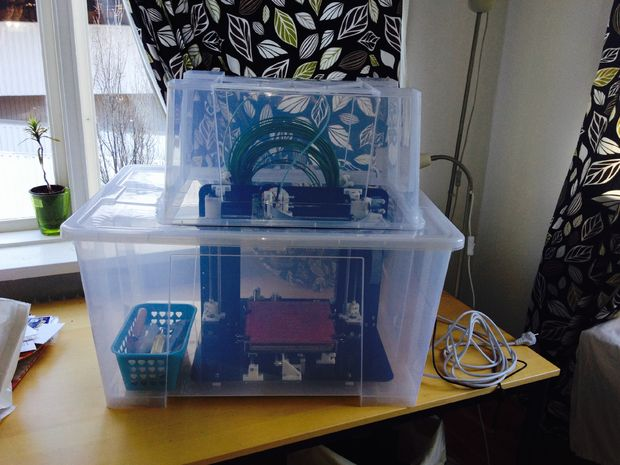
\includegraphics[width=\textwidth,cfbox=azul_marcos 4pt 0pt]{FOTOS/CERRAMIENTO2}
    \end{subfigure}
    \quad %add desired spacing between images, e. g. ~, \quad, \qquad, \hfill etc. 
    %(or a blank line to force the subfigure onto a new line)
    \begin{subfigure}[b]{0.3\textwidth}
        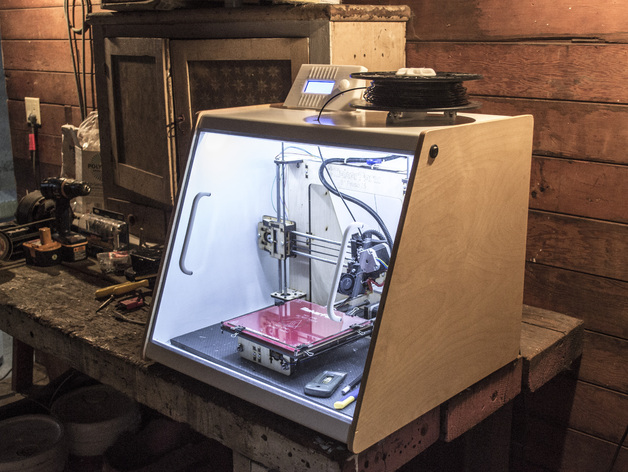
\includegraphics[width=\textwidth,cfbox=azul_marcos 4pt 0pt]{FOTOS/CERRAMIENTO3}
    \end{subfigure}
    \caption*{Exemplos de fechamentos caseiros}
\end{figure}
Por seu turno, são muitas as impressoras que estão concebidas em forma de caixa e que não precisam deste isolamento adicional.
% IMPRESORACERRADA1	IMPRESORACERRADA2	IMPRESORACERRADA3
\begin{figure}[H]
    \centering
    \begin{subfigure}[b]{0.3\textwidth}
        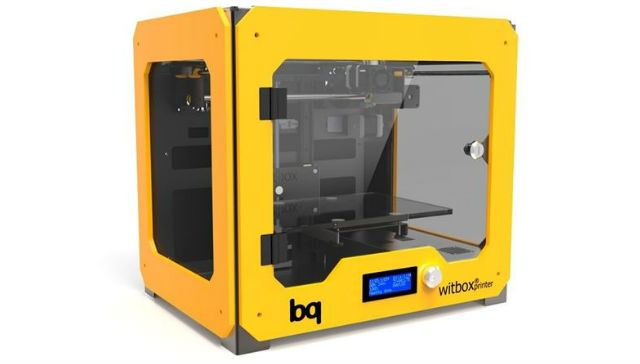
\includegraphics[width=\textwidth,cfbox=azul_marcos 4pt 0pt]{FOTOS/IMPRESORACERRADA1}
    \end{subfigure}
    \quad %add desired spacing between images, e. g. ~, \quad, \qquad, \hfill etc. 
      %(or a blank line to force the subfigure onto a new line)
    \begin{subfigure}[b]{0.3\textwidth}
        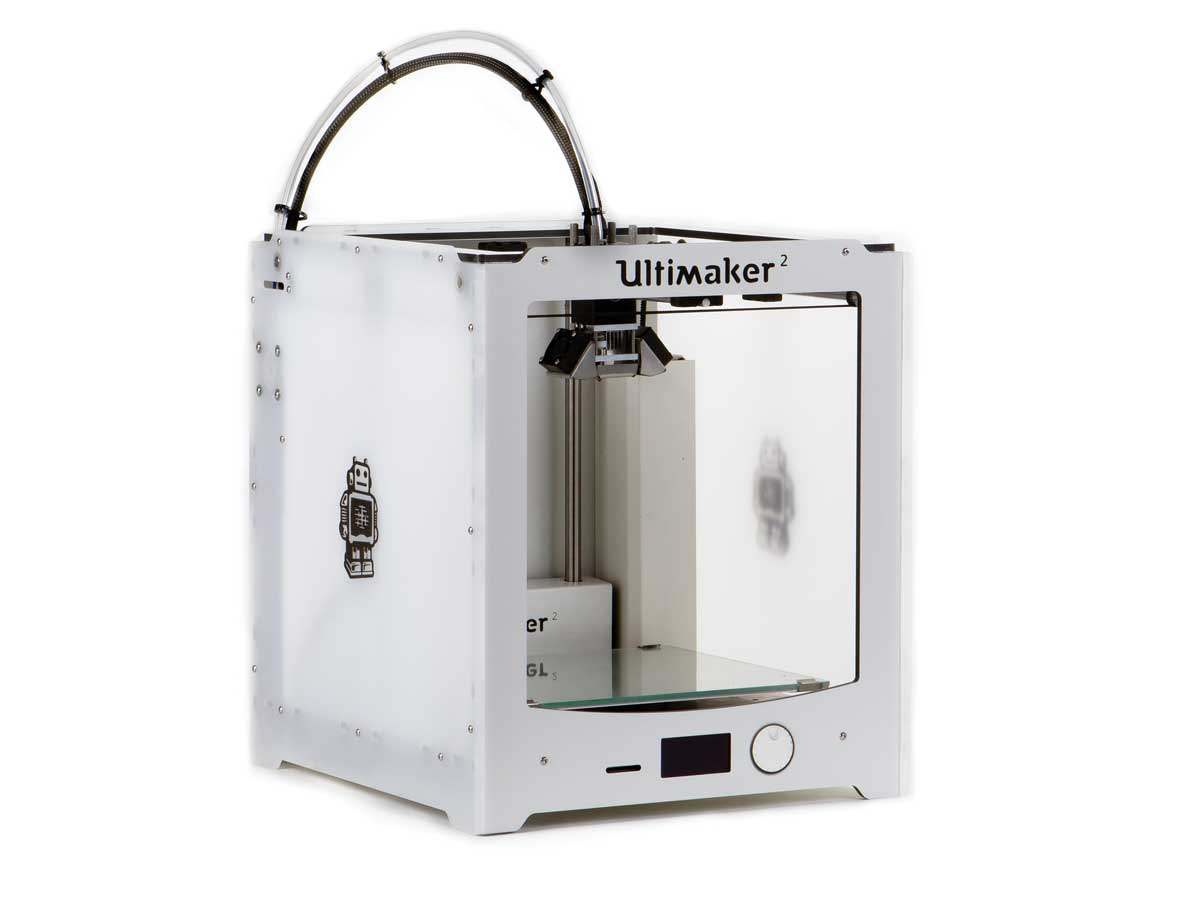
\includegraphics[width=\textwidth,cfbox=azul_marcos 4pt 0pt]{FOTOS/IMPRESORACERRADA2}
    \end{subfigure}
    \quad %add desired spacing between images, e. g. ~, \quad, \qquad, \hfill etc. 
    %(or a blank line to force the subfigure onto a new line)
    \begin{subfigure}[b]{0.3\textwidth}
        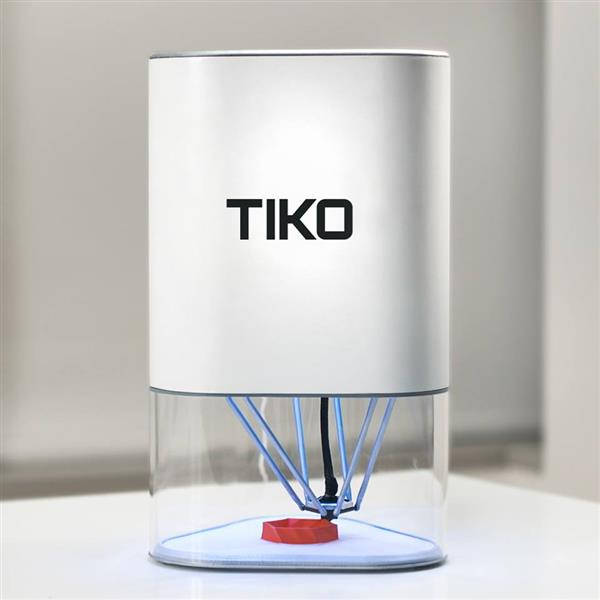
\includegraphics[width=\textwidth,cfbox=azul_marcos 4pt 0pt]{FOTOS/IMPRESORACERRADA3}
    \end{subfigure}
    \caption*{Exemplos de impressoras fechadas}
\end{figure}
			\paragraph{Aquecer o recinto}\mbox{}\\\\
As impressoras industriais e profissionais imprimem ABS num recinto aquecido que mantém a peça a 80º durante toda a impressão. Isto requer engenharia extra para refrigerar o hot-end e o resto dos componentes, mas elimina por completo os problemas de warping e cracking.
\\\\
% STRATASYS
\begin{figure}[H]
\centering
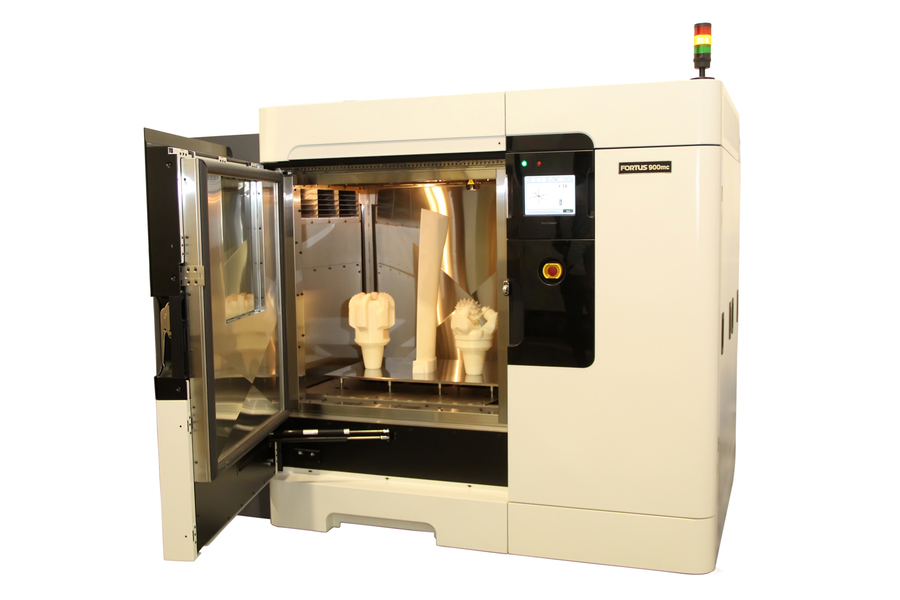
\includegraphics[width=0.6\textwidth,cfbox=azul_marcos 4pt 0pt]{FOTOS/STRATASYS}
\caption*{Impressora industrial com recinto aquecido}
\end{figure}
Apesar de este tipo de impressoras não estar ao alcance do utilizador doméstico, falamos delas para uma melhor compreensão do problema.
		\subsubsection{Soluções de software e de desenho}Além de tudo o que foi comentado anteriormente, existem técnicas de desenho e laminado que permitem reduzir ou eliminar os problemas de warping.
			\paragraph{Brim e raft}\mbox{}\\\\
O brim e o raft são opções oferecidas pelos programas de laminado para aumentar a aderência das peças à base.
%BRIM			RAFT 	
% Leyenda: Brim	Leyenda: Raft
\begin{figure}[H]
    \centering
    \begin{subfigure}[b]{0.4\textwidth}
        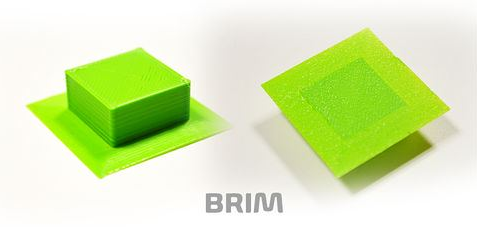
\includegraphics[width=\textwidth,cfbox=azul_marcos 4pt 0pt]{FOTOS/BRIM}
    \end{subfigure}
    \qquad %add desired spacing between images, e. g. ~, \quad, \qquad, \hfill etc. 
      %(or a blank line to force the subfigure onto a new line)
    \begin{subfigure}[b]{0.4\textwidth}
        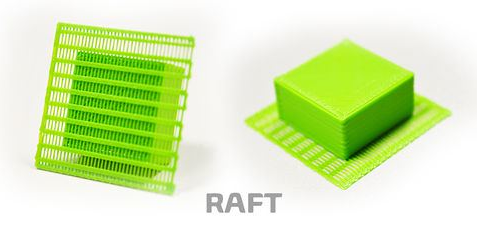
\includegraphics[width=\textwidth,cfbox=azul_marcos 4pt 0pt]{FOTOS/RAFT}
    \end{subfigure}   
\end{figure}
A opção Brim cria perímetros extra em torno da peça para aumentar a superfície e melhorar a adesão.
\\\\
Por seu lado, a opção Raft cria uma espécie de cama de capas com várias espessuras, para depois imprimir a peça sobre a referida cama.
\\\\
Em geral é preferível a utilização de Brim, pois é mais rápido.
\\\\
Para mais informação sobre como ativar e usar estas opções no seu programa de laminado podes consultar os seguintes links:\\\\
\url{http://manual.slic3r.org/expert-mode/skirt}\\\\
\url{https://www.simplify3d.com/support/tutorials/rafts-skirts-and-brims/}\\\\
\url{https://ultimaker.com/en/resources/16525-platform-adhesion}
			\paragraph{Impacto do infill no warping}\mbox{}\\\\
O grau de warping é diretamente proporcional à quantidade de plástico que se contrai, por isso percentagens de infill mais baixas produzem menos warping do que peças com mais enchimento.
\\\\
A dimensão das primeiras capas afeta da mesma maneira que o infill e pode ser recomendável reduzir a espessura ou o número das mesmas.
			\paragraph{Modificação de peças para reduzir o warping}
				\subparagraph{Adicionar suportes nas esquinas}\mbox{}\\\\
Um método de controlar o warping é redesenhar a peça, reforçando os pontos onde se descolou da cama.
\\\\
Se depois de uma impressão falhada verificarmos que uma ou várias esquinas continuam a levantar-se, pode ser necessário adicionar um suporte na referida zona.
\\\\
O suporte deverá ser mais ou menos grande, dependendo da gravidade do problema.
%	MOUSEEAR1			MOUSEEAR2
\begin{figure}[H]
    \centering
    \begin{subfigure}[b]{0.4\textwidth}
        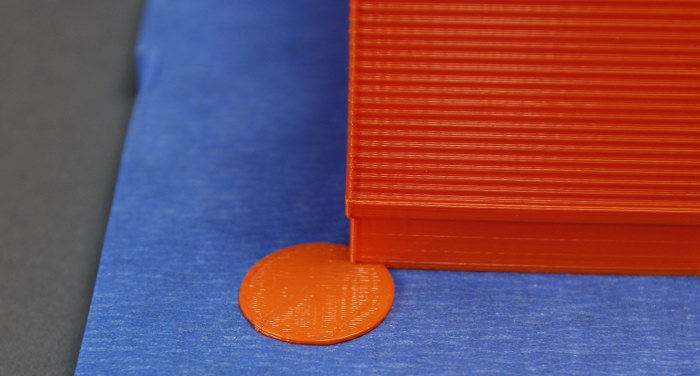
\includegraphics[width=\textwidth,cfbox=azul_marcos 4pt 0pt]{FOTOS/MOUSEEAR1}
    \end{subfigure}
    \qquad %add desired spacing between images, e. g. ~, \quad, \qquad, \hfill etc. 
      %(or a blank line to force the subfigure onto a new line)
    \begin{subfigure}[b]{0.4\textwidth}
        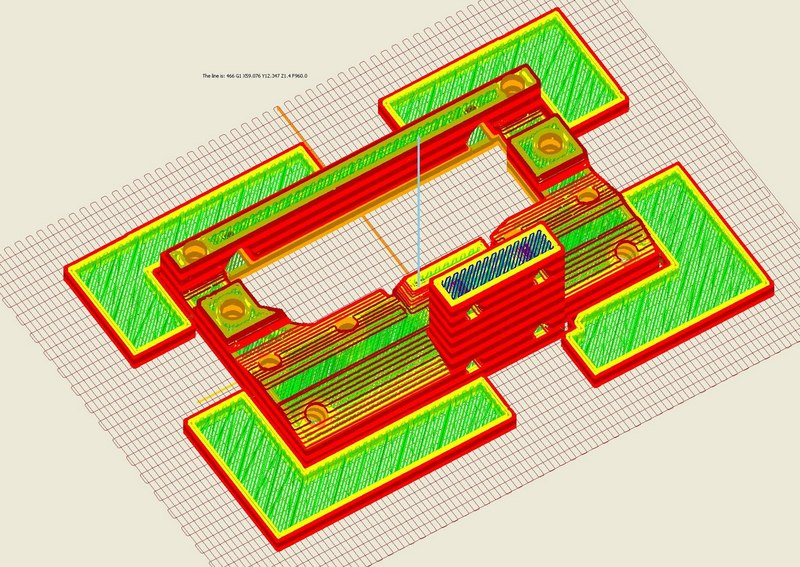
\includegraphics[width=\textwidth,cfbox=azul_marcos 4pt 0pt]{FOTOS/MOUSEEAR2}
    \end{subfigure}   
\end{figure}	
				\subparagraph{Evitar esquinas arredondadas}\mbox{}\\\\
Verificou-se que o warping afeta mais as esquinas redondas e as peças com base circular ou perímetros convexos.
\\\\
Se tem este problema, a sua peça pode ser beneficiada por um redesenho que elimine essas geometrias problemáticas.
			\paragraph{Baixar a velocidade e a altura da primeira capa}\mbox{}\\\\
É muito importante que a primeira capa fique aderida o melhor possível à superfície de impressão.
\\\\
Para o conseguir, é aconselhável reduzir bastante a velocidade da primeira capa, favorecendo uma aderência mais firme e uniforme do material à base.
\\\\
Uma velocidade de 20 mm/s na primeira capa deveria ser suficiente para alcançar aquele objetivo. Também é recomendável reduzir a altura da primeira capa, de forma a não superar os 0.2 mm.
			\paragraph{Uso de ventilador de capa}\mbox{}\\\\
O ventilador de capa encarrega-se de arrefecer o plástico depois da sua extrusão e isto é precisamente o que é preciso evitar ao imprimir ABS.
\\\\
Por isso, como norma geral, é aconselhável desativá-lo para imprimir ABS.
\\\\
Contudo, pode usar-se de forma seletiva em alguns momentos da impressão, se o seu software de laminado permitir.
\\\\
Em todo o caso, se vai utilizá-lo, recomendamos-lhe que o faça a uma velocidade inferior à  habitual.
	\subsection{Os vapores tóxicos}Sabe-se que o ABS emite vapores nocivos ao ser impresso, que podem ser potencialmente prejudiciais para os humanos.
\\\\
Por isso recomenda-se que a impressora esteja num lugar ventilado ou, pelo menos, não se permaneça junto dela de forma prolongada durante o processo de impressão.
\\\\
Se vai utilizar ABS de forma intensiva pode ser interessante instalar um sistema de filtragem e extração na sua impressora para evitar completamente a exposição a estes vapores.
% VENTILACIONVAPORES
\begin{figure}[H]
\centering
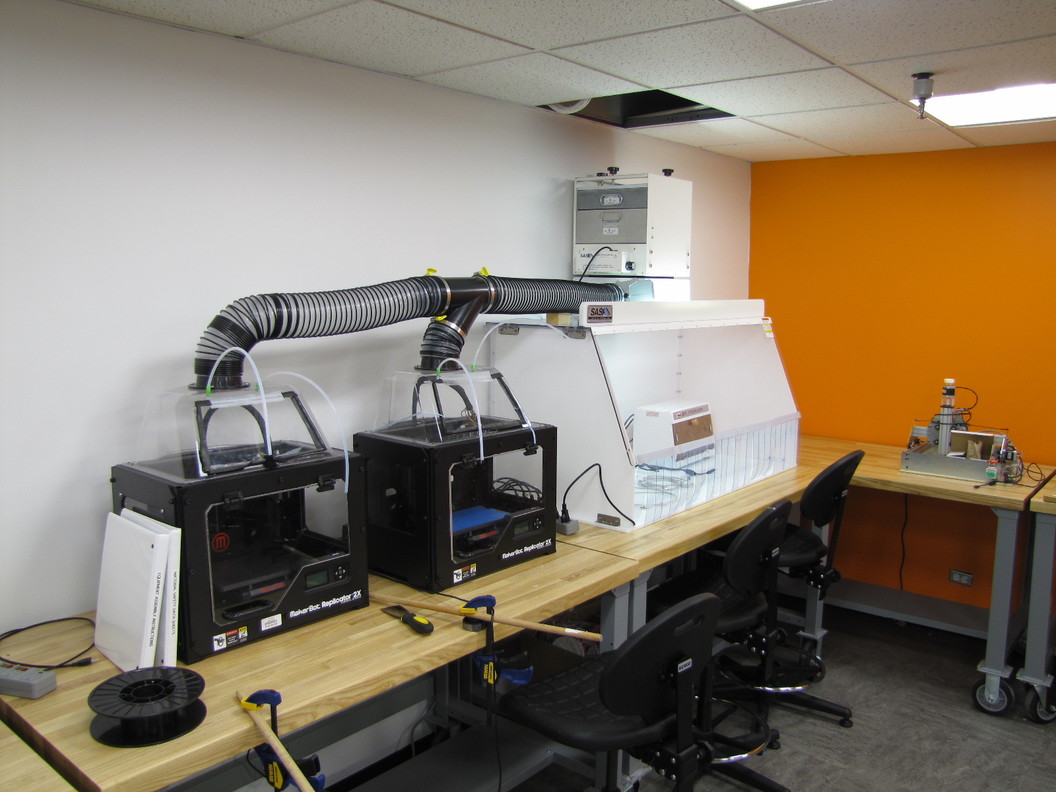
\includegraphics[width=0.5\textwidth,cfbox=azul_marcos 4pt 0pt]{FOTOS/VENTILACIONVAPORES}
\caption*{Sistema de filtragem e extração}
\end{figure}
\section{Conselhos de impressão: O pós-processamento do ABS}
	\subsection{Lixar, cortar e perfurar}Também se pode perfurar sem problemas e pode modelar-se cortando-o com um cutter ou similar.
	\subsection{Pintar}O ABS pode-se pintar com tinta acrílica. É conveniente lixar a superfície da peça para uma melhor fixação da pintura.
	\subsection{Acetona como aglutinante}Como é solúvel em acetona, esta pode ser usada como aglutinante para unir fortemente peças de ABS. Aplicando uma pequena quantidade nas superfícies de contacto, estas irão fundir-se entre si, proporcionando uma união forte e duradoura.
	\subsection{Acetona para polir peças}A acetona também pode ser usada como tratamento superficial, para dar um perfeito aspeto polido e brilhante às peças de ABS. 
% VAPORACETONA1			VAPORACETONA2
\begin{figure}[H]
    \centering
    \begin{subfigure}[b]{0.4\textwidth}
        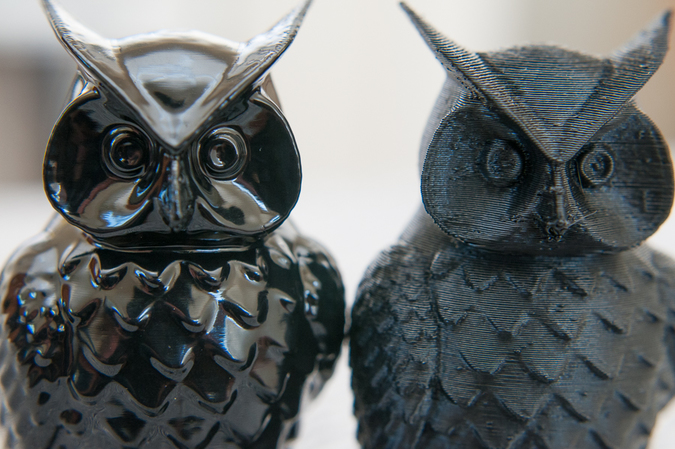
\includegraphics[width=\textwidth,cfbox=azul_marcos 4pt 0pt]{FOTOS/VAPORACETONA1}
    \end{subfigure}
    \qquad %add desired spacing between images, e. g. ~, \quad, \qquad, \hfill etc. 
      %(or a blank line to force the subfigure onto a new line)
    \begin{subfigure}[b]{0.4\textwidth}
        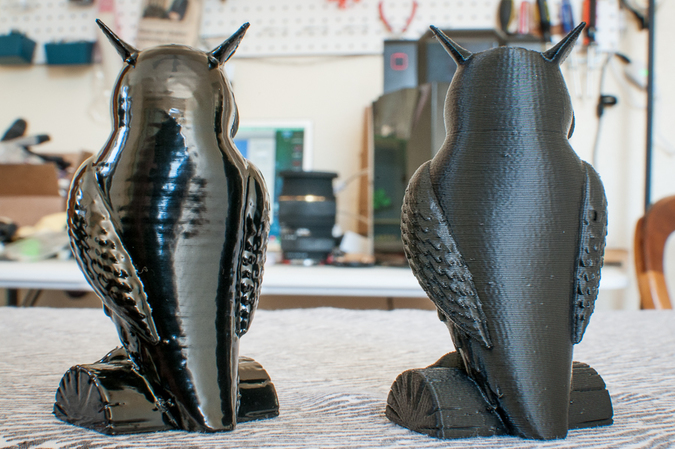
\includegraphics[width=\textwidth,cfbox=azul_marcos 4pt 0pt]{FOTOS/VAPORACETONA2}
    \end{subfigure}   
\end{figure}
Pode ser aplicada à mão, utilizando um pincel, mas também existe a possibilidade de criar uma câmara caseira de vapor de acetona relativamente simples.
\\\\
Nos links seguintes descrevem-se 2 métodos diferentes de impregnar as peças de ABS com vapor de acetona:
\\\\
\url{http://www.instructables.com/id/Safe-way-to-do-Acetone-bath/}\\\\
\url{http://sinkhacks.com/building-acetone-vapor-bath-smoothing-3d-printed-parts/}
\section{Quer apoiar o nosso projeto?}
Todos os membros FFF World adoram a impressão 3D e a comunidade maker. Sentimo-nos uns sortudos por poder trabalhar em projetos onde podemos pôr em prática a nossa paixão sincera. No futuro, gostaríamos de poder desenvolver mais materiais, mais cores, mais formatos. Definitivamente, gostaríamos de poder fazer crescer a nossa empresa.
\\\\
Para isso, uma das principais ações para nos ajudar, se quiser fazê-lo e estiver satisfeito com o filamento, é votar em nós no Amazon com 5 estrelas.
\begin{figure}[H]
\centering

\includegraphics[width=0.5\textwidth,cfbox=azul_marcos 1pt 0pt]{FOTOS/AMAZON_FIVE_STARS}
\caption*{¡Muchas gracias!}
\end{figure}
\subsection{Outros filamentos com excelentes propriedades agora disponíveis no Amazon}
\begin{description}
\item[FlexiSMART Tech:] Concebido para resistir à abrasão e ao desgaste de impressões técnicas.
\item[ABS Tech:] Efeito warping minimizado. Alto rendimento em aplicações técnicas.
\item[PETG Tech:] Máxima resistência mecânica. Resistente ao contacto com a água e os raios UV. Apto para uso alimentar.
\item[FilaMETAL:] PLA com carga metálica não abrasiva que dá um acabamento metálico espetacular às suas impressões.
\item[PC Tech:] Policarbonato com grande resistência à temperatura e com excelentes propriedades mecânicas.
\item[Nylon Tech:] Imprimível a baixa temperatura. Resistência aos choques com um certo grau de flexibilidade.
\item[PVA Tech:] Filamento solúvel em água indicado para ser utilizado como material de suporte. Excelente compatibilidade com PLA.
\item[HIPS Tech:] Filamento solúvel em limoneno, indicado para ser utilizado como material de suporte. Boa resistência mecânica e excelente compatibilidade com ABS.
\end{description}
%\section{Bibliografía}
%Esta guía no habría sido posible sin el conocimiento libre generado por la comunidad RepRap. Para la elaboración de esta guía se han %utilizado imágenes y contenido extraidos de los siguientes sitios web.
%\\\\
%\url{http://www.gyrobot.co.uk/blog/how-to-3d-print-with-flexible-filaments}\\
%\url{http://www.thingiverse.com/thing:1496895}\\
%\url{http://www.thingiverse.com/thing:247024}\\
%\url{http://www.thingiverse.com/thing:16319}\\
%\url{http://www.thingiverse.com/thing:779011}\\
%\url{http://www.thingiverse.com/thing:1102900}\\
%\url{http://www.thingiverse.com/thing:147705}\\
%\url{http://www.thingiverse.com/thing:222667}\\
%\url{http://www.thingiverse.com/thing:512338}\\
%\url{https://all3dp.com/common-3d-printing-problems-and-their-solutions/}\\
%\url{https://www.simplify3d.com/support/}\\
%\url{http://www.thingiverse.com/thing:508896}\\
%\url{http://www.thingiverse.com/thing:1187344}

\includepdf{PDF/PT_CONTRAPORTADA.pdf}
\end{document}
